\section{Semana 9 - CM+Flight Envelope}
Nesta semana foram calculados o centro de massa (CM) e o flight envelope.
\subsection{CM}
O centro de massa foi calculado com base no CAD. No entanto, dado que o CAD foi feito com peças de grossura diferente e geometrias interiores de forma a ter a exterior correta, o centro de massa dado pelo solidworks não se encontra correto. Devido à existência de múltiplas peças maciças perto da cauda, o centro de massa foi trazido para trás. De forma a corrigir tal, foi calculadas as posições de várias secções da aeronave bem como os seus volumes usando simplificações geométricas e a ferramenta de medição interna do solidworks: measure, que se encontra no separador Evaluate.\par
A aeronave foi separada nos seguintes componentes: corpo, asas, e rotores + hélices. Outras partes como aviónica, material médico, etc... foram adicionados no fim dos cálculos. O corpo teve que ser dividido em partes e geometricamente simplificado. Em baixo, observamos o desenho feito à mão realizado para orientar o trabalho e a divisão, juntamente com números sobrepostos a computador de forma a ser possível legendar. Dever-se-á notar o referencial colocado no ponto mais à direita no desenho, isto é, na ponta do cockpit.
\FloatBarrier
\begin{figure}[h]
    \centering
    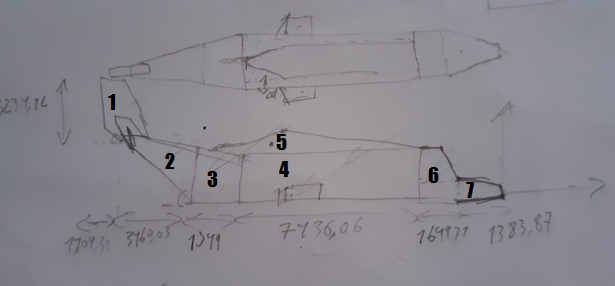
\includegraphics{Imagens/simplificacaoCAD.png}
    \caption{Desenho à mão do corpo da aeronave simplificada}
    \label{draft_aeronave_cad}
\end{figure}
\FloatBarrier
Na figura encontramos as seguintes divisões:
\begin{enumerate*}
    \item Cauda vertical;
    \item Ligação fuselagem cauda - esquerda;
    \item Ligação fuselagem cauda - direita;
    \item Fuselagem;
    \item Turboshaft e Gerador;
    \item Cockpit - esquerda;
    \item Cockpit - direita;
\end{enumerate*}\par
As simplificações foram feitas em CAD para as partes 2,3 e 6, de forma a retirar o centro de massa diretamente do solidworks. A 4 foi considerada um paralelipipedo oco, pelo que o centro de massa pode ser calculado diretamente num excel sem necessidade de realizar outro CAD. O CM da parte 1 foi calculado ao considerar a geometria 2D assumindo o CM no plano de simetria vertical.\par
Apresentamos na figura \ref{cauda2D} a geometria 2D considerada, não desenhada à escala. É constituída por um triângulo, um retângulo e um trapézio. No canto mais à direita, encontra-se representado a origem do referêncial. O CM da cauda foi calculado em relação a este, utilizando as relações usuais de centros geométricos das geometrias anteriormente descritas, sendo que este foi calculado em relação ao referencial da aeronave, utilizando a ferramenta measure.
\FloatBarrier
\begin{figure}[h]
    \centering
    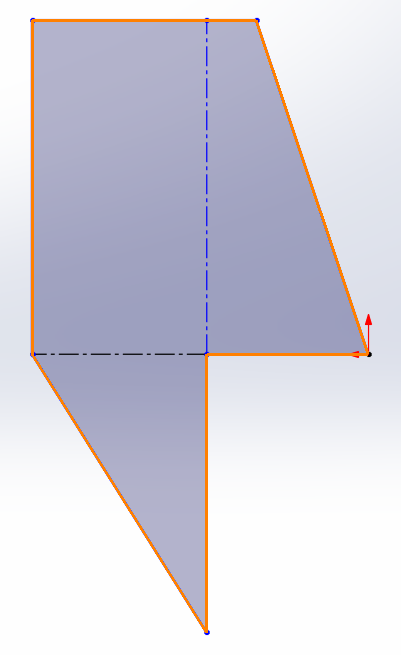
\includegraphics[scale=0.7]{Imagens/cauda2D.PNG}
    \caption{Cauda: geometria 2D (não desenhado à escala)}
    \label{cauda2D}
\end{figure}
\FloatBarrier
Em relação às duas secções que ligam a parte central da fuselagem, 4, à cauda, 1, isto é, as secções 2 e 3, foi modelado em CAD a sua geometria simplificada de forma a ter o CM em relação a um referencial local. Sabendo a posição deste referencial local em relação ao utilizado para a aeronave toda, é possível ter a posição do CM em relação a este também.\par
\FloatBarrier
\begin{figure}[h]
    \centering
    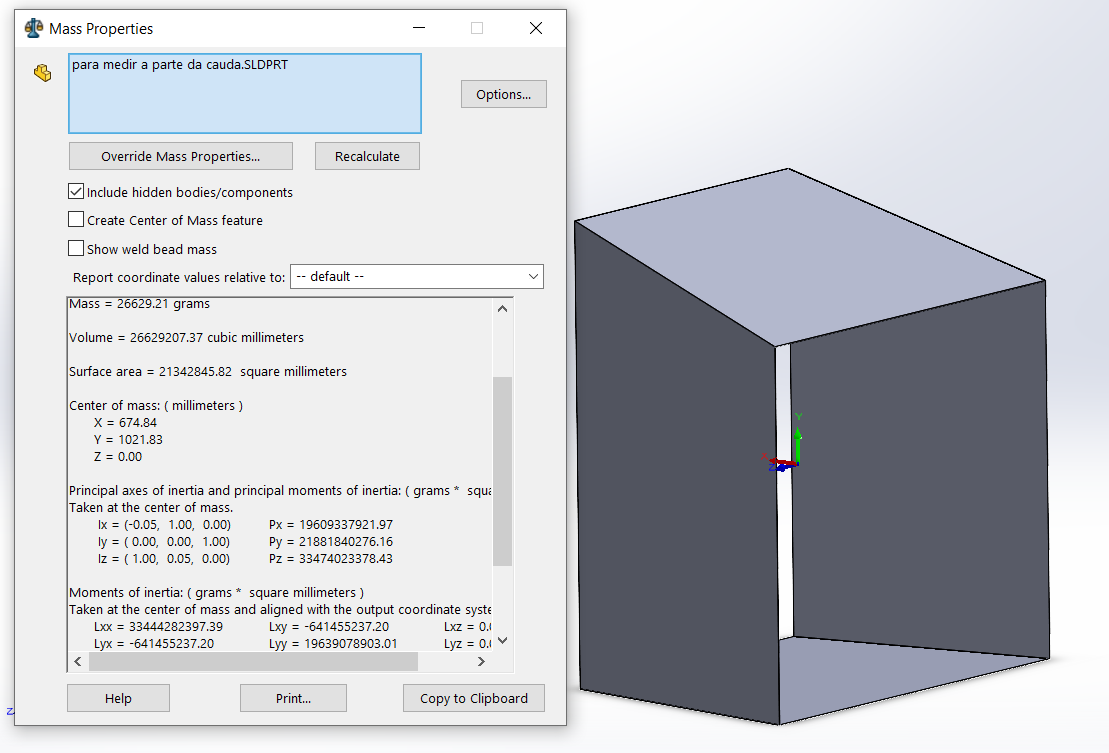
\includegraphics[width=\textwidth]{Imagens/CM_lig_cauda_1.PNG}
    \caption{Peça de ligação - secção 2 - à cauda modelada em 3D com geometria simplificada e seu respetivo centro de massa num referencial local}
    \label{lig_cauda_1}
\end{figure}
\begin{figure}[h]
    \centering
    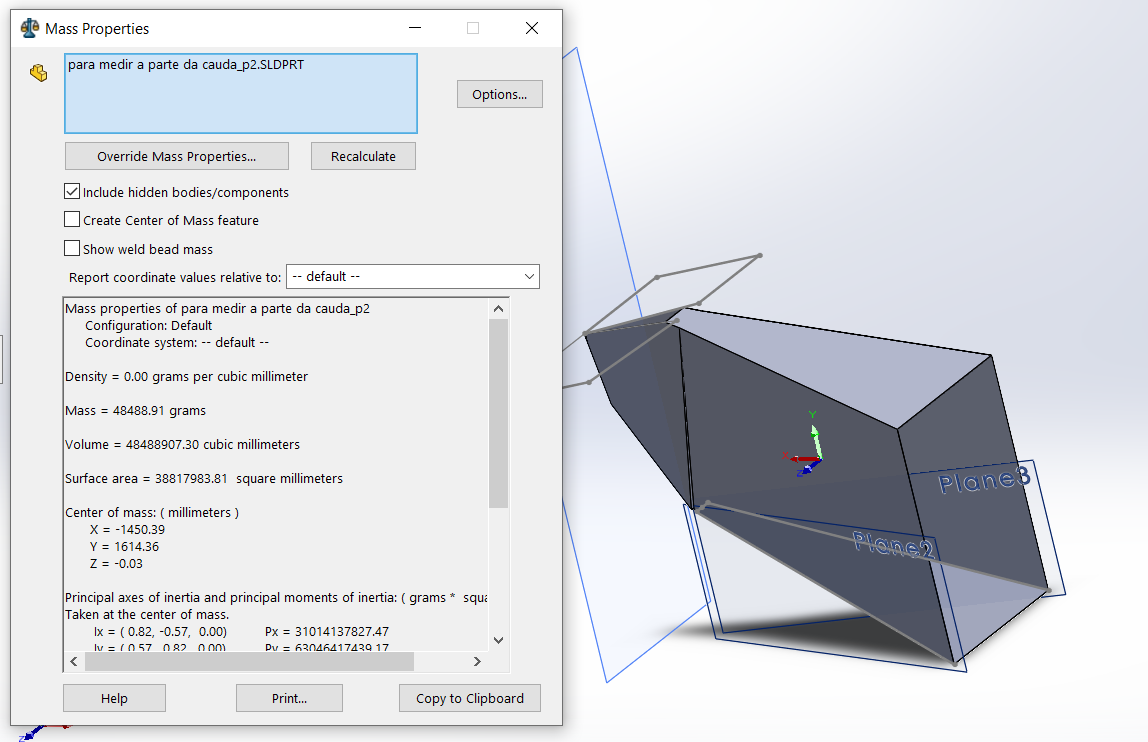
\includegraphics[width=\textwidth]{Imagens/CM_lig_cauda_2.PNG}
    \caption{Peça de ligação - secção 3 - à cauda modelada em 3D com geometria simplificada e seu respetivo centro de massa num referencial local}
    \label{lig_cauda_2}
\end{figure}
\FloatBarrier
Utilizando o mesmo raciocínio, modelou-se o cockpit de igual forma. Notar que foram omitidas as paredes, dado que a geometria é simétrica, pelo que o centro de massa se encontra no mesmo sítio. 
\FloatBarrier
\begin{figure}[h]
    \centering
    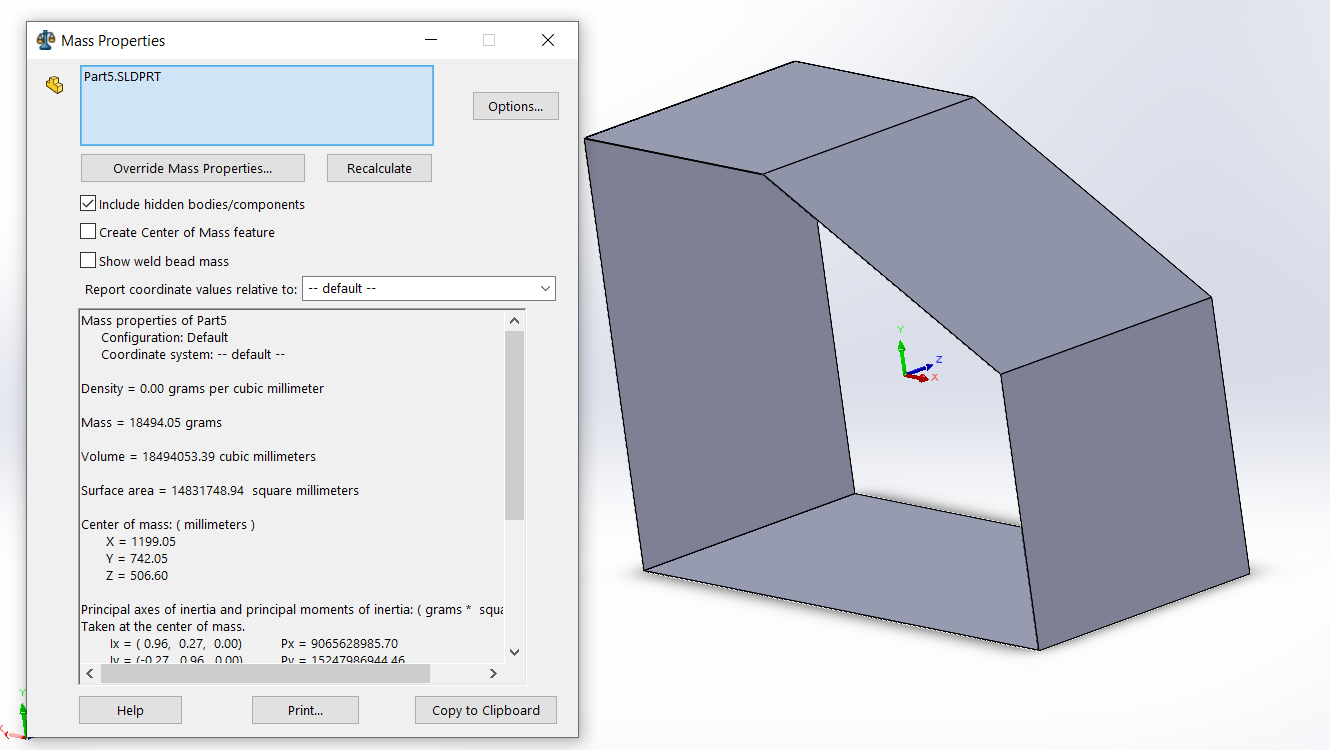
\includegraphics[width=\textwidth]{Imagens/CM_cockpit_1.PNG}
    \caption{Cockpit - secção 6 - modelado em 3D com geometria simplificada e seu respetivo centro de massa num referencial local}
    \label{lig_cauda_1}
\end{figure}
\begin{figure}[h]
    \centering
    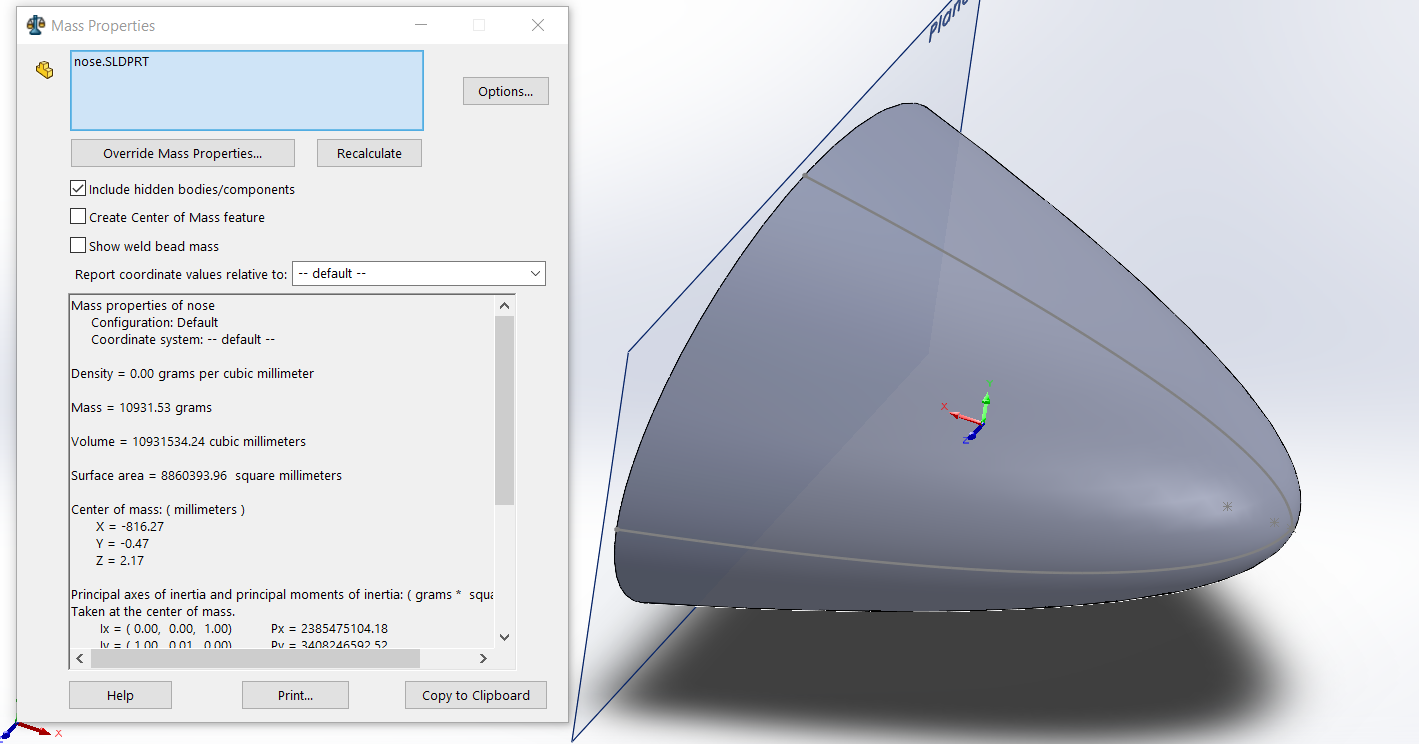
\includegraphics[width=0.80\textwidth]{Imagens/CM_nose.PNG}
    \caption{Nariz - secção 7 - modelado em 3D com geometria simplificada e seu respetivo centro de massa num referencial local}
    \label{lig_cauda_2}
\end{figure}
\FloatBarrier
Estas simplificações permitiram calcular o CM duma fuselagem completamente vazia, sabendo a massa de cada secção. O volume de cada região também foi utilizado para se calcular a massa, sabendo a densidade do material.\par
Tal como já foi referido, materiais interiores à fuselagem fora adicionados igualmente, depois, não sendo necessário ter em conta esses mesmos nos cálculos dos CMs de cada região.\par
Apresentamos, agora, o excel no qual foi calculado o CM. 
\FloatBarrier
\begin{figure}
\centering
    \begin{subfigure}[h]{\textwidth}
        \centering
        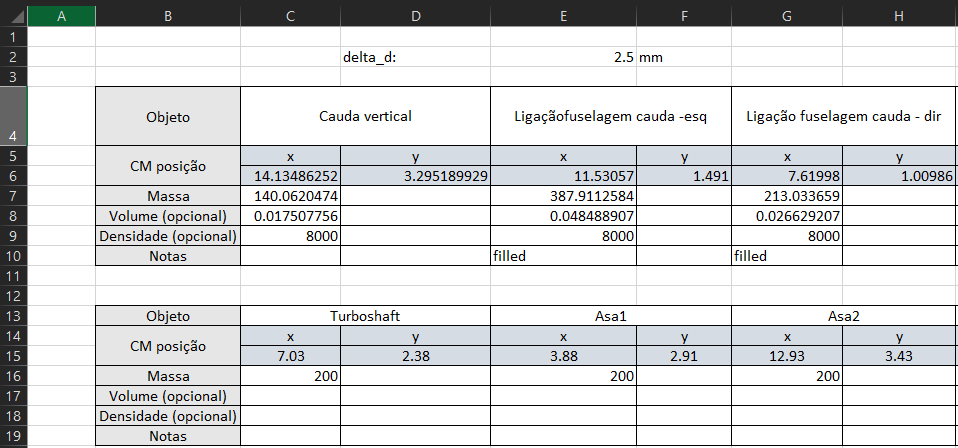
\includegraphics[width=\textwidth]{Imagens/excelp1.PNG}
        \caption{Primeira parte dos cálculos}
        \label{excelCM_p1}
    \end{subfigure}
\end{figure}
\begin{figure}\ContinuedFloat
    \begin{subfigure}[h]{\textwidth}
        \centering
        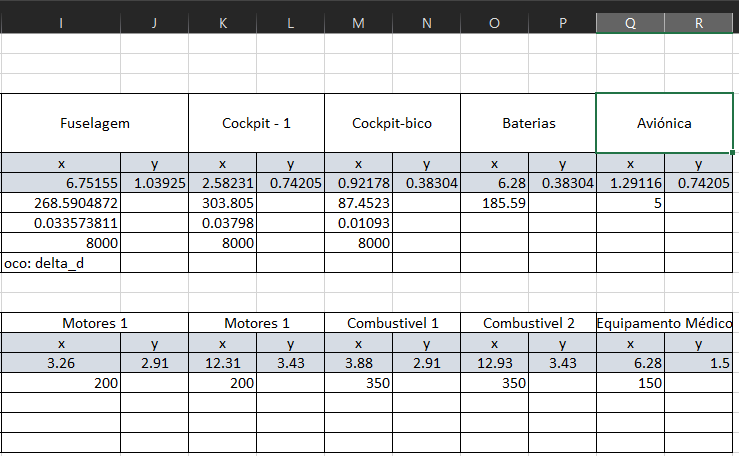
\includegraphics[width=\textwidth]{Imagens/excelp2.PNG}
        \caption{Segunda parte dos cálculos}
        \label{excelCM_p2}
    \end{subfigure}
\end{figure}
\begin{figure}\ContinuedFloat
    \begin{subfigure}[h]{\textwidth}
        \centering
        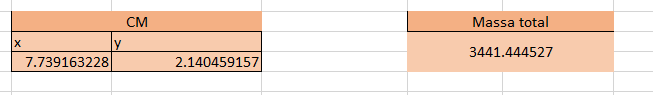
\includegraphics[width=\textwidth]{Imagens/excelp3.PNG}
        \caption{CM final}
        \label{excelCM_p3}
    \end{subfigure}
    \caption{Cálculos do CM da aeronave utilizando Excel}
    \label{excelCM_total}
\end{figure}
\FloatBarrier
O sistema de coordenadas utilizado foi um referencial localizado na ponta mais à frente no nariz do avião, como ser visto na figura \ref{draft_aeronave_cad}, com o eixo x na horizontal a apontar para a cauda, e o eixo y na vertical a apontar para cima. O Excel foi partido em três na figura \ref{excelCM_total} partes de forma a poder ser apresentado numa folha A4.\par
Foi considerada uma grossura de 2.5 nas geometrias da fuselagem, bem como aço como material.